%-------------------------------------------------------------------------------

% This file is part of Code_Saturne, a general-purpose CFD tool.
%
% Copyright (C) 1998-2015 EDF S.A.
%
% This program is free software; you can redistribute it and/or modify it under
% the terms of the GNU General Public License as published by the Free Software
% Foundation; either version 2 of the License, or (at your option) any later
% version.
%
% This program is distributed in the hope that it will be useful, but WITHOUT
% ANY WARRANTY; without even the implied warranty of MERCHANTABILITY or FITNESS
% FOR A PARTICULAR PURPOSE.  See the GNU General Public License for more
% details.
%
% You should have received a copy of the GNU General Public License along with
% this program; if not, write to the Free Software Foundation, Inc., 51 Franklin
% Street, Fifth Floor, Boston, MA 02110-1301, USA.

%-------------------------------------------------------------------------------

\programme{clptrg}


\vspace{1cm}
%%%%%%%%%%%%%%%%%%%%%%%%%%%%%%%%%%
%%%%%%%%%%%%%%%%%%%%%%%%%%%%%%%%%%
\section*{Fonction}
%%%%%%%%%%%%%%%%%%%%%%%%%%%%%%%%%%
%%%%%%%%%%%%%%%%%%%%%%%%%%%%%%%%%%
Ce sous-programme est d�di� au calcul des conditions aux limites en paroi
rugueuse. On utilise le
formalisme introduit dans \var{CONDLI} pour les conditions
aux limites g\'en\'erales.

Par conditions aux limites en paroi, on entend ici l'ensemble des conditions aux
limites pour la vitesse, les grandeurs turbulentes ($k$, $\varepsilon$),
la temp\'erature lorsqu'elle a une valeur de paroi impos\'ee
(ou l'enthalpie et plus g\'en\'eralement les
{\it VarScalaires}\footnote{Comme dans \fort{condli}, on d\'esignera ici par
{\it VarScalaire} toute variable solution
d'une \'equation de convection-diffusion autre que la
vitesse, la pression et les grandeurs turbulentes $k$, $\varepsilon$. La
d\'enomination {\it VarScalaire} pourra en particulier se rapporter
\`a la temp\'erature, \`a l'enthalpie ou \`a un scalaire passif.}
\`a traiter en paroi en prenant en compte une loi de similitude
pour la couche limite associ\'ee). Pour les {\it VarScalaires}, en particulier,
lorsque les conditions aux limites de paroi sont du type Neumann (homog\`ene ou non),
elles sont trait\'ees dans \fort{condli} et on ne s'y int\'eresse donc pas
ici. En particulier, les conditions aux limites des  {\it VarScalaires}
repr\'esentant la variance de fluctuations d'autres  {\it VarScalaires} ne
sont pas trait\'ees ici car leur traitement en paroi est de type Neumann homog\`ene.

On indique comment sont calcul\'es les couples de coefficients
$A_b$ et $B_b$ qui sont utilis\'es pour le calcul de certains
termes discrets des \'equations \`a r\'esoudre et qui
permettent  en particulier de d\'eterminer une valeur associ\'ee aux faces
de bord $f_{b,int}$ (en un point localis\'e au ``centre'' de la face de bord,
barycentre de ses sommets) par la
relation $f_{b,int} = A_b+B_b\,f_{I'}$ ($f_{I'}$ est la valeur de
la variable au point
$I'$, projet\'e du centre de la cellule jouxtant le bord sur la droite
normale \`a
la face de bord et passant par son centre~: voir la figure~\ref{fig_flux_clptur}).

\begin{figure}[h]
\centerline{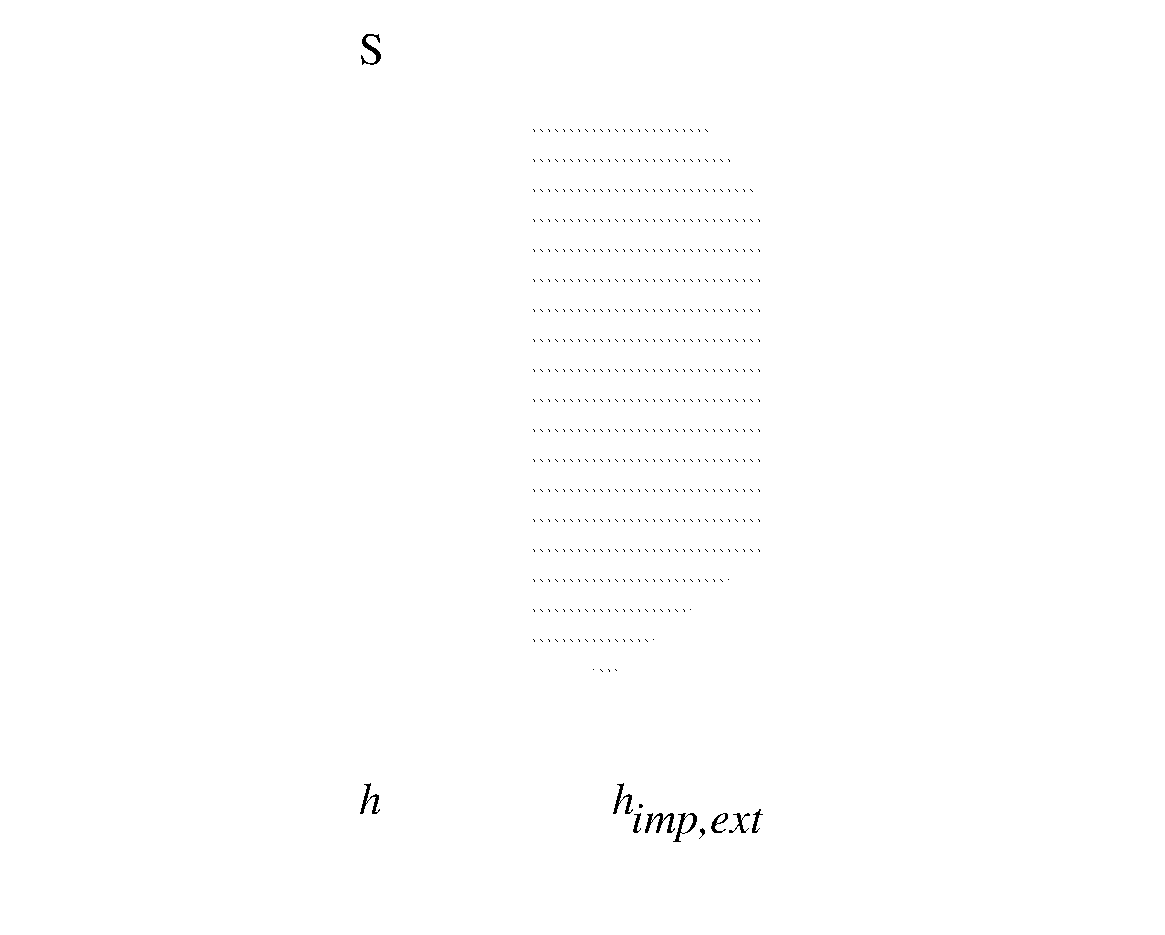
\includegraphics[height=7cm]{fluxbord}}
\caption{\label{fig_flux_clptur}Cellule de bord.}
\end{figure}

%%%%%%%%%%%%%%%%%%%%%%%%%%%%%%%%%%
%%%%%%%%%%%%%%%%%%%%%%%%%%%%%%%%%%
\section*{Discr\'etisation}
%%%%%%%%%%%%%%%%%%%%%%%%%%%%%%%%%%
%%%%%%%%%%%%%%%%%%%%%%%%%%%%%%%%%%

\etape{Notations\vspace{0,3cm}}
%%%%%%%%%%%%%%%%%%%%%%%%%%%%%%%%%%%%%%%%%%%%%%%%%%%%%%%%%%%%%%%%%%%%%%%%%%%%%%%
La vitesse de la paroi est not\'ee
$\vect{v}_p$. On la suppose projet\'ee dans le plan tangent \`a la paroi (si
elle ne l'est pas, le code la projette).

La vitesse du fluide est not\'ee $\vect{u}$. L'indice $I$, $I'$ ou $F$ d\'esigne le
point auquel elle est estim\'ee. La composante tangentielle par rapport \`a la
paroi est not\'ee $u_\tau$.
 La vitesse du fluide dans le rep\`ere li\'e \`a la paroi (vitesse
``relative'') est not\'ee $\vect{u}^r=\vect{u} - \vect{v}_p$.

Le rep\`ere orthonorm\'e li\'e \`a la paroi est not\'e
$\hat {\mathcal R}=(\vect{\tau},\vect{\tilde{n}},\vect{b})$.
\begin{itemize}
\item [$\bullet$] $\vect{\tilde{n}}=-\vect{n}$ est le vecteur norm\'e
orthogonal \`a la paroi et dirig\'e vers l'int\'erieur du domaine de calcul.
\item [$\bullet$] $\vect{\tau} = \displaystyle\frac{1}{\|\vect{u}^r_{I'}-(\vect{u}^r_{I'}\,.\,\vect{\tilde{n}})\|}\left[\vect{u}^r_{I'}-(\vect{u}^r_{I'}\,.\,\vect{\tilde{n}})\right]$ est le vecteur norm\'e port\'e par la projection de la vitesse
relative en $I'$, $\vect{u}^r_{I'}$, dans le plan tangent \`a la
paroi ({\it i.e.} orthogonal \`a $\vect{\tilde{n}}$)~: voir la
figure~\ref{fig_flux_clptur}.
\item [$\bullet$] $\vect{b}$ est le vecteur norm\'e compl\'etant le rep\`ere direct.
\end{itemize}

\vspace{0.5cm}

Dans le cas du {\bf mod\`ele \`a deux  \'echelles de vitesse}, on note~:
\begin{itemize}
\item [-] $u_k$ la
vitesse de frottement en paroi obtenue \`a partir de l'\'energie turbulente.

\item [-] $u^*$ la vitesse de frottement en paroi d\'etermin\'ee \`a
partir de la relation $ \displaystyle\frac{u^r_{\tau,I'}}{u^*} = f(z_p)$.

\item [-] $z_p$  repr�sente une distance � la paroi
      (c'est � dire la distance depuis le bord du domaine de calcul),  soit
$z_p= I'F$ (voir la figure~\ref{fig_flux_clptur}). La fonction $f$ traduit la forme id�ale du profil de
      vitesse. Dans l'atmosph�re, cette fonction est donn�e par
      une loi de type logarithmique faisant intervenir la rugosit� dynamique de
      la paroi $z_0$~:

$f(z_p)= \displaystyle\frac{1}{\kappa} ln \left ( \displaystyle \frac
      {z_p+z_0}{z_0} \right ) $


\item [-] Les deux \'echelles de vitesse $u_k$ et $u^*$ sont simples \`a
      calculer mais leur obtention
n\'ecessite la connaissance de l'\'energie turbulente $k_I$ au centre de la
maille jouxtant la face de bord.

\item [-] Le mod\`ele \`a deux \'echelles
est le mod\`ele par d\'efaut dans \CS. Il permet souvent, et en particulier
dans les cas avec transfert thermique, de diminuer les effets de certains
d\'efaut li\'es au mod\`ele $k-\varepsilon$ (exemple classique du jet impactant).
\end{itemize}

On se sert plus bas de $u^*$ et $u_k$ pour les conditions aux limites portant
sur la vitesse et les scalaires (temp\'erature en particulier).


\begin{equation}
\label{Eq_Mod_'2ech_Vit}
\begin{array}{l}
\text{\bf Mod\`ele \`a deux \'echelles de vitesse}\\
\left\{\begin{array}{l}
u_k = C_\mu^\frac{1}{4}k_I^\frac{1}{2}\\
u^* \text{solution de }  \displaystyle\frac{u^r_{\tau,I'}}{u^*} =
\displaystyle\frac{1}{\kappa}ln(z_k)\\
z_k=\displaystyle\frac{I'F+z_0}{z_0} = \displaystyle\frac{z_p+z_0}{z_0}\\
\text{   avec   } C_\mu =0,09 \text{  et }  \kappa = 0,42
\end{array}\right.\\
\end{array}
\end{equation}


\vspace{0.5cm}

Dans le cas du {\bf mod\`ele \`a une \'echelle de vitesse}, on note $u^*$ l'unique vitesse
de frottement en paroi solution de l'\'equation
$\displaystyle\frac{u^r_{\tau,I'}}{u^*} = f(z_p)$. La grandeur
$z_p$  repr\'esente une distance \`a la paroi, soit
$z_p=I'F$. La fonction $f$ traduit la forme id\'eale du profil de vitesse comme
pour le mod\`ele \`a deux \'echelles de vitesses. On peut
noter que cette vitesse de frottement, d'un calcul plus d\'elicat (point fixe),
s'obtient  cependant sans faire r\'ef\'erence aux
variables turbulentes ($k$, $\varepsilon$). Par commodit\'e, on posera
dans le cas du mod\`ele \`a une \'echelle $u_k=u^*$.

On se sert plus bas de $u^*$ et $u_k$ pour les conditions aux limites portant
sur la vitesse et les scalaires (temp\'erature en particulier).

\begin{equation}
\begin{array}{l}
\text{\bf Mod\`ele \`a une \'echelle de vitesse}\\
\left\{\begin{array}{l}
u_k = u^*\\
u^* \text{solution de }  \displaystyle\frac{u^r_{\tau,I'}}{u^*} =
\displaystyle\frac{1}{\kappa}ln(z_k)\\
z_k=\displaystyle\frac{I'F+z_0}{z_0} = \displaystyle\frac{z_p+z_0}{z_0}\\
\text{   avec   } C_\mu =0,09 \text{  et }  \kappa = 0,42
\end{array}\right.\\
\end{array}
\end{equation}

\etape{Conditions aux limites pour la vitesse en $k-\varepsilon$\vspace{0,3cm}}
%%%%%%%%%%%%%%%%%%%%%%%%%%%%%%%%%%%%%%%%%%%%%%%%%%%%%%%%%%%%%%%%%%%%%%%%%%%%%%%
On consid\`ere tout d'abord les conditions utilis\'ees dans le cas d'un calcul
r\'ealis\'e avec le mod\`ele $k-\varepsilon$. Ce sont en effet les plus
complexes et les plus g\'en\'erales.

Les conditions aux limites sont n�cessaires pour imposer au bord la contrainte
tangentielle $\sigma_\tau=\rho_Iu^*u_k$ ad�quate dans l'\'equation de  quantit\'e de
mouvement\footnote{Proposition de modification des conditions aux limites de
paroi turbulente pour le Solveur Commun dans le cadre du mod\`ele
$k-\varepsilon$ standard, rapport EDF HI-81/00/019/A, 2000, M. Boucker, J.-D. Mattei.}
($\rho_I$ est la masse volumique au centre de la
cellule $I$). Le terme qui n\'ecessite des conditions aux limites est celui qui contient la
d\'eriv\'ee de la vitesse dans la direction normale \`a la paroi,
soit\footnote{Le terme en gradient transpos\'e est trait\'e dans \fort{visecv}
et ne sera pas consid\'er\'e ici.}~:
$(\mu_I+\mu_{t,I})\ggrad{\vect{u}}\,\vect{n}$. Il appara\^\i t au second membre
de l'\'equation de quantit\'e de mouvement usuelle (voir \fort{bilsc2} et \fort{predvv}).

Dans le cas o\`u le mod\`ele $k-\varepsilon$ a tendance \`a surestimer la
production de l'\'energie turbulente, l'\'echelle de longueur du mod\`ele,
$L_{k-\varepsilon}$,
peut devenir significativement plus grande que l'\'echelle th\'eorique maximale
des tourbillons de la couche limite turbulente $L_{\text{th\'eo}}$. On note :
\begin{equation}
\left\{\begin{array}{l}
L_{k-\varepsilon} = C_{\mu}\displaystyle\frac{k^\frac{3}{2}}{\varepsilon}\\
L_{\text{th\'eo}} = \kappa\, \left( I'F+z_0 \right) = \kappa\, \left(z_p+z_0 \right)
\end{array}\right.
\end{equation}

Dans le cas o\`u $L_{k-\varepsilon}>L_{\text{th\'eo}}$, on a donc
$\mu_{t,I}>\mu_{t}^{lm}$ avec $\mu_{t,I}$ la viscosit\'e turbulente du mod\`ele
$k-\varepsilon$ au point $I$ et $\mu_{t}^{lm}=\rho_I L_{\text{th\'eo}}u_k$ la
viscosit\'e turbulente du mod\`ele de longueur de m\'elange. En outre, la
contrainte tangentielle peut s'\'ecrire en faisant appara\^\i tre la viscosit\'e
turbulente, soit~:
\begin{equation}
\sigma_\tau = \rho_Iu^*u_k = \displaystyle\frac{u^*}{\kappa\,
 \left(I'F+z_0 \right)}
\underbrace{\rho_I\kappa\, \left( I'F+z_0 \right)  u_k}_{\mu^{lm}_t}
\end{equation}
L'\'echelle de viscosit\'e introduite dans la contrainte est alors en
contradiction avec celle d\'eduite de la turbulence calcul\'ee alentour par le
mod\`ele. On pr\'ef\`ere d\`es lors \'ecrire, en utilisant l'\'echelle de
longueur du $k-\varepsilon$ chaque fois qu'elle est inf\'erieure \`a la limite
$L_{\text{th\'eo}}$~:
\begin{equation}
\sigma_\tau = \displaystyle\frac{u^*}{\kappa\, \left(I'F+z_0 \right)} max(\mu_{t}^{lm},\mu_{t,I})
\end{equation}

On peut alors utiliser cette valeur  pour le calcul du flux
diffusif qui en d\'epend dans l'\'equation de Navier-Stokes~:
\begin{equation}\label{eq_grad_sigma_clptur}
(\mu_I+\mu_{t,I})\ggrad{\vect{u}}\,\vect{n}=-\sigma_\tau \vect{\tau}
\end{equation}

Or, le gradient de vitesse (gradient \`a la face de bord) est calcul\'e dans le
code sous la forme suivante~:
\begin{equation}\label{eq_grad_uf_clptur}
(\mu_I+\mu_{t,I})\ggrad{\vect{u}}\,\vect{n}=
\displaystyle\frac{(\mu_I+\mu_{t,I})}{\overline{I'F}}(\vect{u}_F-\vect{u}_{I'})
\end{equation}

Du rapprochement de (\ref{eq_grad_sigma_clptur}) et de
(\ref{eq_grad_uf_clptur}) on tire alors la valeur de $\vect{u}_F$ \`a
imposer, soit $\vect{u}_{F,flux}$~(respect du flux de quantit\'e de mouvement)~:
\begin{equation}\label{eq_uf_flux_clptur}
\begin{array}{ll}
\vect{u}_{F,flux}&=\vect{u}_{I'}-\displaystyle\frac{\overline{I'F}}{\mu_I+\mu_{t,I}}\sigma_\tau \vect{\tau}\\
                 &=\vect{u}_{I'}-\displaystyle\frac{u^*}{\kappa\,
		  (\mu_I+\mu_{t,I})} max(\mu_{t}^{lm},\mu_{t,I})
		  \, \displaystyle\frac {I'F} {\left(I'F+z_0 \right)} \vect{\tau}
\end{array}
\end{equation}

En r\'ealit\'e, une approximation suppl\'ementaire est r\'ealis\'ee, qui
consiste \`a imposer la vitesse normale nulle \`a la paroi et \`a utiliser
l'\'equation (\ref{eq_uf_flux_clptur}) projet\'ee sur le plan tangent \`a la
paroi, soit~:
\begin{equation}
\vect{u}_{F,flux}=\left[u_{\tau,I'}-\displaystyle\frac{u^*}{\kappa\,
(\mu_I+\mu_{t,I})} max(\mu_{t}^{lm},\mu_{t,I}) \, \displaystyle\frac {I'F} {\left(I'F+z_0 \right)} \right]\vect{\tau}
\end{equation}

Enfin, on peut \'egalement faire appara\^\i tre la vitesse de la paroi
dans l'expression finale~:
\begin{equation}
\begin{array}{l}
\text{\bf Conditions aux limites sur la vitesse de type ``flux''}\,(k-\varepsilon)\\
\left\{\begin{array}{l}
\vect{u}_{F,flux}=\vect{v}_p+\left[u^r_{\tau,I'}-\displaystyle\frac{u^*}{\kappa\,
(\mu_I+\mu_{t,I})} max(\mu_{t}^{lm},\mu_{t,I})  \, \displaystyle\frac {I'F} {\left(I'F+z_0 \right)}\right]\vect{\tau}
\end{array}\right.\\
\end{array}
\end{equation}

Un premier couple de coefficients $A_{flux}$ et $B_{flux}$ s'en d\'eduit (pour
chaque composante de vitesse s\'epar\'ement) et il n'est utilis\'e que pour le
calcul du terme d\'ependant de la contrainte tangentielle (voir \fort{bilsc2})~:
\begin{equation}
\begin{array}{l}
\text{\bf Coefficients associ\'es aux conditions aux limites sur la vitesse de
type ``flux''} (k-\varepsilon)\\
\left\{\begin{array}{l}
\vect{A}_{flux}=\vect{v}_p+\left[u^r_{\tau,I'}-\displaystyle\frac{u^*}{\kappa\,
(\mu_I+\mu_{t,I})} max(\mu_{t}^{lm},\mu_{t,I}) \, \displaystyle\frac {I'F} {\left(I'F+z_0 \right)} \right]\vect{\tau} \\
\vect{B}_{flux} = \vect{0}
\end{array}\right.
\end{array}
\end{equation}

On a vu ci-dessus comment imposer une condition \`a la limite permettant de
calculer correctement le terme en contrainte. Une analyse suppl\'ementaire est
n\'ecessaire pour le calcul des gradients de vitesse. On cherche \`a trouver une
valeur en face de bord qui permette d'obtenir, avec la formulation adopt\'ee pour le gradient, la valeur de la production turbulente la
plus proche possible de la valeur th\'eorique, elle-m\^eme d\'etermin\'ee
en utilisant la loi
logarithmique, pour \'evaluer la d\'eriv\'ee normale de la vitesse tangentielle.
Ainsi, on d\'efinit (au point $I$)~:
\begin{equation}\label{eq_ptheo_clptur}
P_{\text{th\'eo}} = \rho_I u^* u_k
\|\displaystyle\frac{\partial u_\tau}{\partial\vect{n}}\|_{I} =
\rho_I \displaystyle\frac{u_k(u^*)^2}{\kappa\, \left(I'F+z_0 \right)}
\end{equation}

Par ailleurs, le terme pr\'epond\'erant de la production calcul\'ee dans la
cellule $I$ est, pour les situations classiques ($z$ est l'ordonn\'ee sur l'axe
de vecteur directeur $\vect{\tilde{n}}$),
\begin{equation}
P_{\text{calc}} =
\mu_{t,I}\left(\displaystyle\frac{\partial u_\tau}{\partial z}\right)^2_{I}
\end{equation}

\begin{figure}[h]
\centerline{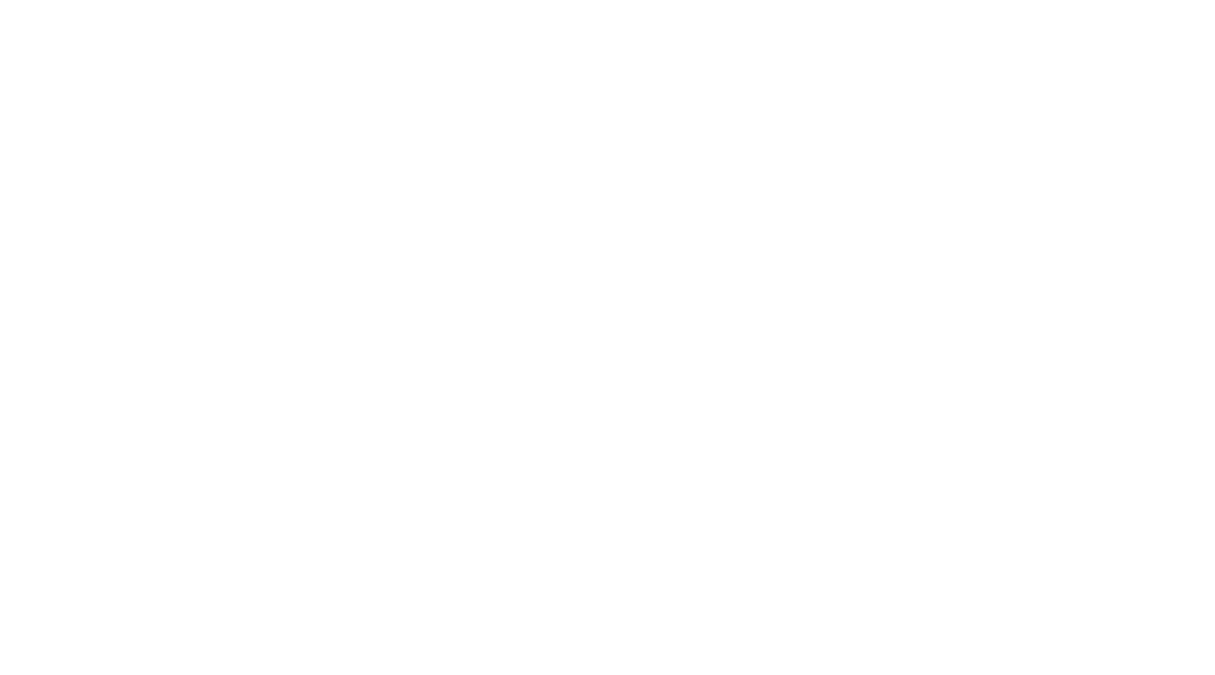
\includegraphics[height=7cm]{bordortho}}
\caption{\label{fig_bord_ortho_clptur}Cellule de bord - Maillage orthogonal.}
\end{figure}

Or, le gradient normal de la vitesse tangentielle (gradient cellule) est
calcul\'e dans le code en volumes finis et son expression dans le cas d'un
maillage orthogonal et r\'egulier est la suivante (voir les notations sur la figure~\ref{fig_bord_ortho_clptur})~:
\begin{equation}
P_{\text{calc}} =
\mu_{t,I}\left(\displaystyle\frac{u_{\tau,G}-u_{\tau,F}}{2d}\right)^2 =
\mu_{t,I}\left(\displaystyle\frac{u_{\tau,I}+u_{\tau,J}-2u_{\tau,F}}{4d}\right)^2
\end{equation}
On suppose alors que $u_{\tau,J}$ peut \^etre obtenu \`a partir de $u_{\tau,I}$
et du gradient normal de $u_{\tau}$ \'evalu\'e en G \`a partir de la loi
logarithmique, soit~:
\begin{equation}
\label{eq_dvp_lim_utau}
u_{\tau,J}=u_{\tau,I}+ IJ\,.\,(\partial_z u_{\tau})_G+\mathcal{O} (IJ^{\,2}) \approx
u_{\tau,I}+ IJ\,.\,\left[\partial_z \left(\displaystyle
\frac{u^*}{\kappa}\,ln{ (z)} \right)\right]_G=
u_{\tau,I}+2d \, \displaystyle\frac{u^*}{\kappa \left(2d + z_0\right)}
\end{equation}
et l'on obtient alors~:
\begin{equation}\label{eq_pcalc_clptur}
\begin{array}{lll}
P_{\text{calc}}
&=&\mu_{t,I}\left(\displaystyle\frac{2u_{\tau,I}+2d  \, \displaystyle\frac{\,u^*}{\kappa
	     \left(2d + z_0\right) } -2u_{\tau,F}}{4d}\right)^2 \\
&=&
\mu_{t,I}\left(\displaystyle\frac{u_{\tau,I}+d \,\displaystyle\frac{\,u^*}{\kappa
	  \left(2d + z_0\right)} -u_{\tau,F}}{2d}\right)^2
\end{array}
\end{equation}

On rapproche alors les \'equations (\ref{eq_ptheo_clptur}) et
(\ref{eq_pcalc_clptur}) pour imposer que la production calcul\'ee soit \'egale
\`a la la production th\'eorique. On \'etend sans pr\'ecaution les formules
pr\'ec\'edentes aux maillages non orthogonaux (la vitesse en $I$ est
alors simplement prise en $I'$).
On obtient alors l'expression suivante pour $u_{\tau,F}$~:
\begin{equation}
u_{\tau,F,grad} =u_{\tau,I'}-\displaystyle\frac{u^*}{\kappa}\left(
2d\sqrt{\displaystyle\frac{\rho_I\kappa\, u_k }{\mu_{t,I} \left(I'F
							   +z_0\right) }
}-\displaystyle\frac{1}{2 + z_0/I'F}\right)
\end{equation}

On impose d'autre part que le gradient reste au moins aussi raide que celui
donn\'e par la d\'eriv\'ee normale du profil de vitesse th\'eorique
(logarithmique) en $I'$~:\\
$\partial_z u_{\tau} = \partial_z (\displaystyle
\frac{u^*}{\kappa}\,ln{ (z)} ) =\displaystyle\frac{u^*}{\kappa\,\left(I'F + z_0\right) }$, soit
donc~:
\begin{equation}
u_{\tau,F,grad} =u_{\tau,I'}-\displaystyle\frac{u^*}{\kappa}max\left(1,
2d\sqrt{\displaystyle\frac{\rho_I\kappa\, u_k }{\mu_{t,I} \left(I'F + z_0\right)}}-\displaystyle\frac{1}{2 + z_0/I'F}\right)
\end{equation}


La vitesse normale \`a la paroi est impos\'ee nulle.
De plus, si la vitesse tangentielle en $I'$ est
nulle (de valeur absolue inf\'erieure \`a une limite num\'erique arbitraire de
$10^{-12}$) une condition d'adh\'erence est appliqu\'ee. Enfin, on peut
\'egalement faire appara\^\i tre la vitesse de la paroi dans l'expression finale~:
\begin{equation}
\begin{array}{l}
\text{\bf Conditions aux limites sur la vitesse de type ``gradient''} (k-\varepsilon)\\
\left\{\begin{array}{l}
\vect{u}_{F,grad}=\vect{v}_p
          \qquad\qquad\text{ si } u^r_{\tau,I'} < 10^{-12}  \\
\vect{u}_{F,grad}=\vect{v}_p +
u^r_{\tau,I'}-\displaystyle\frac{u^*}{\kappa}\left[max\left(1,2d\sqrt{\displaystyle\frac{\rho_I\kappa\, u_k }{\mu_{t,I}
\left(I'F + z_0\right)}}-\displaystyle\frac{1}{2 + z_0/I'F}\right)\right] \vect{\tau}
\end{array}\right.
\end{array}
\end{equation}

Un second couple de coefficients $A_{grad}$ et $B_{grad}$ s'en d\'eduit (pour
chaque composante de vitesse s\'epar\'ement) et est utilis\'e chaque fois que le
gradient de la vitesse est n\'ecessaire (hormis pour les termes d\'ependant de
la contrainte tangentielle, trait\'es dans \fort{bilsc2} au moyen des
coefficients $A_{flux}$ et $B_{flux}$)~:
\begin{equation}
\begin{array}{l}
\text{\bf Coefficients associ\'es aux conditions aux limites sur la vitesse }\\
\qquad\qquad\qquad\qquad\text{\bf de type ``gradient''} (k-\varepsilon)\\
\left\{\begin{array}{l}
\vect{A}_{grad}=\vect{v}_p
                    \qquad\qquad\text{ \ si\ } u^r_{\tau,I'} < 10^{-12}  \\
\vect{A}_{grad}=\vect{v}_p+
 u^r_{\tau,I'}-\displaystyle\frac{u^*}{\kappa}\left[max\left(1,2d\sqrt{\displaystyle\frac{\rho_I\kappa\, u_k }{\mu_{t,I}
\left(I'F + z_0\right)}}-\displaystyle\frac{1}{2 + z_0/I'F}\right)\right] \vect{\tau}\\
\vect{B}_{grad} = \vect{0}
\end{array}\right.
\end{array}
\end{equation}

\newpage

\etape{Conditions aux limites pour les variables $k$ et $\varepsilon$ (mod\`ele
$k-\varepsilon$ standard)\vspace{0,3cm}}

On impose sur $k$ une condition de Dirichlet tir\'ee de la vitesse de frottement
$u_k$ (se reporter \`a l'\'equation~(\ref{Eq_Mod_'2ech_Vit})), soit :
\begin{equation}
k= \displaystyle\frac{u_k^2}{C_\mu^\frac{1}{2}}
\end{equation}


On cherche \`a imposer la d\'eriv\'ee normale de $\varepsilon$ \`a partir de la
loi th\'eorique suivante (voir les notations sur la figure \ref{fig_bord_ortho_clptur})~:
\begin{equation}\label{eq_partialep_theo_clptur}
G_{\text{th\'eo},\varepsilon} = \displaystyle\frac{\partial}{\partial z}
 \left[ \displaystyle\frac{u_k^3}{\kappa\, \left(z + z_0\right)}\right]
\end{equation}



On utilise le point $M$ pour imposer une condition \`a la limite avec un ordre plus
\'elev\'e en espace. En effet, la simple utilisation de la relation
$\varepsilon_F=\varepsilon_I+d\partial_z\varepsilon_I + O(d^2)$ conduit \`a une
pr\'ecision d'ordre 1.
En utilisant les d\'eveloppements limit\'es suivants, on peut
obtenir une pr\'ecision \`a l'ordre 2~:
\begin{equation}
\left\{\begin{array}{ll}
\varepsilon_M&=\varepsilon_I-\displaystyle\frac{d}{2}\partial_z\varepsilon_I+\displaystyle\frac{d^2}{8}\partial^2_z\varepsilon_I+O(d^3)\\
\varepsilon_M&=\varepsilon_F+\displaystyle\frac{d}{2}\partial_z\varepsilon_F+\displaystyle\frac{d^2}{8}\partial^2_z\varepsilon_F+O(d^3)
\end{array}\right.
\end{equation}
Par diff\'erence, ces relations conduisent \`a
\begin{equation}\label{eq_epsf_clptur}
\varepsilon_F=\varepsilon_I-\displaystyle\frac{d}{2}(\partial_z\varepsilon_I+\partial_z\varepsilon_F)+O(d^3)
\end{equation}
De plus, on a
\begin{equation}
\left\{\begin{array}{ll}
\partial_z\varepsilon_I&=\partial_z\varepsilon_M+d\partial^2_z\varepsilon_M+O(d^2)\\
\partial_z\varepsilon_F&=\partial_z\varepsilon_M-d\partial^2_z\varepsilon_M+O(d^2)
\end{array}\right.
\end{equation}
La somme de ces deux derni\`eres relations permet d'\'etablir
$\partial_z\varepsilon_I+\partial_z\varepsilon_F=2\partial_z\varepsilon_M+O(d^2)$ et, en reportant dans
(\ref{eq_epsf_clptur}), on obtient alors une expression de $\varepsilon_F$ \`a
l'ordre 2, comme souhait\'e~:
\begin{equation}
\varepsilon_F=\varepsilon_I-d\partial_z\varepsilon_M+O(d^3)
\end{equation}
On utilise alors la valeur th\'eorique (\ref{eq_partialep_theo_clptur}) pour
\'evaluer $\partial_z\varepsilon_M$ et on obtient alors la valeur \`a imposer au bord ($d=I'F$)~:
\begin{equation}
\varepsilon_F=\varepsilon_I+d\displaystyle\frac{ u_k^3}{\kappa\, (d/2+ z_0)^2}
\end{equation}


Cette relation est \'etendue au cas de maillages non orthogonaux sans
pr\'ecaution (ce qui doit d\'egrader l'ordre en espace).

On a finalement~:

\begin{equation}
\begin{array}{l}
\text{\bf Conditions aux limites sur les variables } k \text { \bf et } \varepsilon \\
\left\{\begin{array}{ll}
k_F&= \displaystyle\frac{u_k^2}{C_\mu^\frac{1}{2}}\\
\varepsilon_F&=\varepsilon_{I'}+I'F\displaystyle\frac{ u_k^3}{\kappa\,
 (I'F/2 + z_0)^2}
\end{array}\right. \\
\end{array}
\end{equation}
et les coefficients associ\'es
\begin{equation}
\begin{array}{l}
\text{\bf Coefficients associ\'es aux conditions aux limites sur les variables }
k \text { \bf et } \varepsilon \\
\left\{\begin{array}{llll}
A_k&= \displaystyle\frac{u_k^2}{C_\mu^\frac{1}{2}} &\text{ et } B_k&= 0 \\
A_\varepsilon&=I'F\displaystyle\frac{ u_k^3}{\kappa\, (I'F/2 + z_0)^2}&\text{ et } B_\varepsilon&= 1
\end{array}\right.\\
\end{array}
\end{equation}

\newpage
\etape{Conditions aux limites pour les {\it VarScalaires}\vspace{0,3cm}}
On ne traite ici que les conditions se pr\'esentant sous la forme d'une valeur
impos\'ee (\`a la paroi ou en retrait de celle-ci avec un coefficient
d'\'echange externe \'eventuel). On se reporte aux notations de la figure
\ref{fig_flux_clptur} et \`a la pr\'esentation g\'en\'erale disponible dans
\fort{condli} dont on ne reprend que la partie essentielle ci-dessous.

La conservation du flux normal au bord pour la variable $f$ s'\'ecrit sous la forme~:
\begin{equation}\label{eq_flux_clptur}
\begin{array}{l}
    \underbrace{h_{int}(f_{b,int}-f_{I'})}_{\phi_{int}}
  = \underbrace{h_{b}(f_{b,ext}-f_{I'})}_{\phi_{b}}
  = \left\{\begin{array}{ll}
    \underbrace{h_{imp,ext}(f_{imp,ext}-f_{b,ext})}_{\phi_{\text{\it r\'eel
impos\'e}}} &\text{(condition de Dirichlet)}\\
    \underbrace{\phi_{\text{\it imp,ext}}}_{\phi_{\text{\it r\'eel impos\'e}}}
            &\text{(condition de Neumann)}
           \end{array}\right.
\end{array}
\end{equation}


On r\'earrange ces deux \'equations afin d'obtenir la valeur num\'erique
$f_{b,int}=f_{F}$ \`a imposer en face de paroi, \'etant donn\'ees les valeurs de
$f_{imp,ext}$ et de $h_{imp,ext}$ fix\'ees par l'utilisateur et la valeur $h_{b}$
dict\'ee par les lois de similitude qui seront d\'etaill\'ees plus bas. On
pr\'ecise les coefficients $A$ et $B$ qui s'en d\'eduisent naturellement.

\begin{equation}\label{eq_fbint_clptur}
\begin{array}{l}
\text{\bf Conditions aux limites sur les {\it VarScalaires} }\\
f_{b,int} =
\underbrace{\displaystyle\frac{h_{imp,ext}}{h_{int}+h_r h_{imp,ext} } f_{imp,ext}}_{A} +
\underbrace{\displaystyle\frac{h_{int}+h_{imp,ext}(h_r-1)}{h_{int}+h_r h_{imp,ext} }}_{B} f_{I'}
\text{  avec } h_r=\displaystyle\frac{h_{int}}{h_{b}}
\end{array}
\end{equation}


\newpage
{\bf Principe de similitude~: calcul de } $h_b$.

Dans l'expression (\ref{eq_fbint_clptur}), seule reste �
d\'eterminer la valeur de $h_{b}$, celle de $h_{int}$ \'etant une valeur
num\'erique coh\'erente avec le mode de calcul des gradients aux faces et
pr\'ecis\'ee dans \fort{condli} ($h_{int}=\displaystyle\frac{\alpha}{\overline{I'F}}$). La
valeur de  $h_{b}$ doit permettre de
relier le flux \`a l'\'ecart entre les valeurs $f_{I'}$ et $f_{b,ext}$ en
prenant en compte la couche limite (le profil de $f$ n'est pas toujours
lin\'eaire)~:
\begin{equation}
\phi_b=h_b\,(f_{b,ext}-f_{I'})
\end{equation}

Les consid\'erations suivantes sont pr\'esent\'ees en adoptant des notations
g\'en\'erales. En particulier, le nombre de Prandtl-Schmidt est not\'e
$\sigma=\displaystyle\frac{\nu\,\rho\,C}{\alpha}$.
Lorsque le scalaire $f$ consid\'er\'e est la temp\'erature,
on a (voir \fort{condli})~:
\begin{list}{$\bullet$}{}
\item $C=C_p$ (chaleur massique),
\item $\alpha=\lambda$ (conductivit\'e mol\'eculaire),
\item $\sigma = \displaystyle\frac{\nu\,\rho\,C_p}{\lambda} = Pr$
       (nombre de Prandtl),
\item $\sigma_t = Pr_t$ (nombre de Prandtl turbulent),
\item $\phi=\left(\lambda+\displaystyle\frac{C_p\mu_t}{\sigma_t}\right)
        \displaystyle\frac{\partial T}{\partial z}$ (flux en $Wm^{-2}$).
\end{list}

On s'est appuy� sur la r\'ef\'erence "The atmospheric boundary layer",
J. R. Garratt, Cambridge University Press.

Le flux en paroi s'�crit, pour le scalaire $f$ (le flux est positif s'il est
entrant dans le domaine fluide, comme l'indique l'orientation de l'axe $z$)~:
\begin{equation}\label{Eq_Flux_scalaire}
\phi = -\left(\alpha+C\,\frac{\mu_t}{\sigma_t}\right)
                  \frac{\partial f}{\partial z}
     = -\rho\,C \left(\displaystyle\frac{\alpha}{\rho\,C}+
                                \frac{\mu_t}{\rho\sigma_t}\right)
                  \frac{\partial f}{\partial z}
\end{equation}

\noindent Pour la temp�rature, avec $a=\displaystyle\frac{\lambda}{\rho\,C_p}$ et
$a_t=\displaystyle\frac{\mu_t}{\rho\,\sigma_t}$,
on a donc, de mani�re �quivalente~:
\begin{equation}
\phi = -\rho\,C_p(a+a_t)\frac{\partial T}{\partial z}
\end{equation}

\noindent On introduit $f^*$ afin d'adimensionner $f$, en utilisant la valeur du flux
au bord $\phi_b$~:
\begin{equation}
f^* = -\displaystyle\frac{\phi_b}{\rho\,C\,u_k}
\end{equation}
Pour la temp\'erature, on a donc~:
\begin{equation}
T^* = -\displaystyle\frac{\phi_b}{\rho\,C_p\,u_k}
\end{equation}

\noindent On rappelle que dans le cas du  mod\`ele \`a deux  \'echelles de vitesse,  $u_k$ est la
vitesse de frottement en paroi obtenue \`a partir de l'\'energie
cin�tique moyenne du mouvement turbulent\footnote{$u_k = C_\mu^\frac{1}{4}k_I^\frac{1}{2}$}. Dans le
cas du  mod�le � une �chelle de vitesse, on pose $u_k=u^*$ avec $u^*$
la vitesse de frottement en paroi d�termin�e � partir de la loi logarithmique.

On divise alors les membres de l'\'equation~(\ref{Eq_Flux_scalaire})
par $\phi_b$. Pour le membre de gauche, on simplifie en utilisant le fait
que le flux se conserve et donc que $\phi=\phi_b$. Pour le membre de droite,
on remplace $\phi_b$ par sa valeur $-\rho\,C\,u_k\,f^*$. Avec les notations~:
\begin{equation}
       \nu=\displaystyle\frac{\mu}{\rho}
\qquad \nu_t=\displaystyle\frac{\mu_t}{\rho}
\qquad f^+=\displaystyle\frac{f-f_{b,ext}}{f^*}
\end{equation}
on a~:
\begin{equation}\label{Eq_Flux_scalaire_adim}
1 =  \left(\displaystyle\frac{\nu}{\sigma}+
              \displaystyle\frac{\nu_t} {\sigma_t}\right)
                  \displaystyle\frac{\partial f^+}{\partial z} \displaystyle\frac{1}{u_k}
\end{equation}

Remarquons d\`es \`a pr\'esent qu'avec les notations pr\'ec\'edentes,
$h_b$ s'exprime en fonction de $f^+_{I'}$~:
\begin{equation}
h_b=\displaystyle\frac{\phi_b}{f_{b,ext}-f_{I'}}=\frac{\rho\,C\,u_k}{f^+_{I'}}
\end{equation}

Pour d\'eterminer $h_b$, on int\`egre alors
l'\'equation~(\ref{Eq_Flux_scalaire_adim}) afin de disposer de $f^+_{I'}$.
L'unique difficult\'e consiste alors \`a prescrire une loi de variation de
$\mathcal{K}=\displaystyle\frac{\nu}{\sigma}+
              \displaystyle\frac{\nu_t} {\sigma_t}$


Dans la zone turbulente pleinement d�velopp\'ee, une hypoth\`ese de
longueur de m\'elange permet de mod\'eliser les variations de $\nu_t$~:
\begin{equation}
\nu_t = l^2 \arrowvert \frac{\partial U}{\partial z} \arrowvert =
\kappa\,u^* \left(z + z_0\right)
\end{equation}
De plus, les effets de diffusion de $f$
(ou effets "conductifs" lorsque $f$ repr\'esente la temp\'erature)
sont n\'egligeables devant les effets turbulents~: on n\'eglige alors
$\displaystyle\frac{\nu}{\sigma}$ devant
$\displaystyle\frac{\nu_t}{\sigma_t}$. On a donc
finalement~:
\begin{equation}
\mathcal{K}= \displaystyle\frac{\kappa \,u_k}{\sigma_t}  \left(z+z_0\right)
\end{equation}


On int\`egre l'�quation adimensionnelle~(\ref{Eq_Flux_scalaire_adim})
sous la m\^eme hypoth\`ese et on obtient alors la loi donnant $f^+$~:
\begin{equation}
f^+ = \displaystyle\frac{\sigma_t}{\kappa}\,
        ln\left(\displaystyle\frac{z+z_0}{z_{o_T}}\right)
\end{equation}
o� $z_{o_T}$ est la longueur de rugosit� thermique. Son ordre de
grandeur compar� � la rugosit� dynamique  est donn� par la
relation $ln\left(\displaystyle\frac{z_0}{z_{o_T}}\right) \approx 2$ (r�f�rence J. R. Garratt).

Pour r\'esumer, le calcul de $h_b$ est r\'ealis\'e en d\'eterminant~:
\begin{eqnarray}
f^+_{I'}&=& \displaystyle\frac{\sigma_t}{\kappa}\,
 ln\left(\displaystyle\frac{I'F+z_0}{z_{o_T}}\right) \\
h_b&=&\displaystyle\frac{\phi_b}{f_{b,ext}-f_{I'}}=\frac{\rho\,C\,u_k}{f^+_{I'}}
\end{eqnarray}


%%%%%%%%%%%%%%%%%%%%%%%%%%%%%%%%%%
%%%%%%%%%%%%%%%%%%%%%%%%%%%%%%%%%%
\section*{Mise en \oe uvre}
%%%%%%%%%%%%%%%%%%%%%%%%%%%%%%%%%%
%%%%%%%%%%%%%%%%%%%%%%%%%%%%%%%%%%

%\etape{Mode de prescription des conditions aux limites\vspace{0,3cm}}
%%%%%%%%%%%%%%%%%%%%%%%%%%%%%%%%%%%%%%%%%%%%%%%%%%%%%%%%%%%%%%%%%%%%
On traite ici les variables \var{IVAR} sur les faces \var{IFAC}
telles que \var{ICODCL(IFAC,IVAR)}=5.

La vitesse de d\'efilement (\'eventuellement nulle) de la paroi est tout d'abord
projet\'ee dans le plan tangent \`a la paroi. Ses trois composantes dans le
rep\`ere de calcul sont stock\'ees dans les
tableaux\\  \var{RCODCL(IFAC,IUIPH,1),RCODCL(IFAC,IVIPH,1)RCODCL(IFAC,IWIPH,1)}.

On d\'etermine ensuite le
rep\`ere local $\hat{\mathcal R}$. Pour chaque face, il est disponible dans les
vecteurs $\vect{\tau}$ \var{(TX, TY, TZ)}, $\vect{\tilde{n}}$ \var{(-RNX, -RNY,
-RNZ)}, et $\vect{b}$ \var{(T2X, -T2Y,-T2Z)}. Par ailleurs, si la norme de la vitesse
tangentielle est inf\'erieure \`a la valeur arbitraire \var{EPZERO}
($10^{-12}$), l'indicateur \var{TXN0} est positionn\'e \`a 0 (il vaut 1 sinon)
et le vecteur $\vect{\tau}$ est pris
\begin{itemize}
\item [-] arbitraire, dans le plan perpendiculaire \`a $\vect{\tilde{n}}$ en
$R_{ij}-\varepsilon$  (on utilise les composantes de $\vect{\tilde{n}}$ pour
construire  $\vect{\tau}$~; si  $\vect{\tilde{n}}$ est identiquement nul, le
code s'arr\^ete)~;
\item [-] identiquement nul sinon.
\end{itemize}

On calcule ensuite les vitesses de frottement qui sont stock\'ees dans
\var{UET} ($=u^*$) et dans \var{UK} ($=u_k$). Le sous-programme \fort{atmcls}
 permet de calculer la vitesse de
frottement pour le mod\`ele \`a une \'echelle
de vitesse (\var{IDEUCH}=0). Pour le mod\`ele \`a deux \'echelles
(\var{IDEUCH}=1), le calcul (plus simple) de \var{UET} et de \var{UK} est fait directement
dans \fort{clptur}.

Dans le cas ou le mod\`ele \`a une \'echelle de vitesse est actif, on impose
\var{UK=UET} afin de conserver la coh\'erence du codage dans la suite du
sous-programme.

Les conditions aux limites pour la vitesse sont ensuite compl\'et\'ees.
\begin{itemize}

\item [-] En $k-\varepsilon$, on affecte, pour les trois composantes de vitesse
respectivement, \`a $$\var{COEFA(IFAC,ICLU)}, \var{COEFA(IFAC,ICLV)} \,\text{ et
}\,\var{COEFA(IFAC,ICLW)}$$ les coefficients $A_{flux}$
issus de l'analyse relative \`a la contrainte tangentielle.\\
 De m\^eme, les coefficients $B_{flux}$ sont affect\'es \`a
$$\var{COEFB(IFAC,ICLU)}, \var{COEFB(IFAC,ICLV)} \,\text{ et
}\,\var{COEFB(IFAC,ICLW)}.$$ Les conditions aux limites
issues de l'analyse portant directement sur le gradient de vitesse $A_{grad}$ et
$B_{grad}$ sont affect\'ees \`a  $$\var{COEFA(IFAC,ICLUF)},
\var{COEFA(IFAC,ICLVF)}, \var{COEFA(IFAC,ICLWF)}$$ et
$$\var{COEFB(IFAC,ICLUF)}, \var{COEFB(IFAC,ICLVF)}, \var{COEFB(IFAC,ICLWF)}.$$

\item [-] Lorsque la vitesse tangentielle en $I'$ est inf\'erieure \`a
\var{EPZERO}, l'indicateur \var{TXN0} est annul\'e (sinon,  \var{TXN0} vaut 1).
 Cet  indicateur est utilis\'e pour annuler les coefficients $A$ et
      imposer des conditions d'adh\'erence.

\item [-] la vitesse de d\'efilement de la paroi est prise en compte dans les
conditions aux limites (coefficients \var{COEFA}).

\end{itemize}

Les conditions sur les grandeurs turbulentes sont ensuite
compl\'et\'ees.


Les conditions aux limites pour les scalaires sont ensuite compl\'et\'ees. Les
coefficients \var{COEFA} et \var{COEFB} sont simplement renseign\'es en
utilisant les conditions aux limites d\'ecrites pr\'ec\'edemment. La seule
difficult\'e consiste \`a g\'erer correctement les diff\'erentes grandeurs
permettant de  calculer le coefficient d'\'echange $h_b$ sans erreur.

L'indicateur \var{ISCSTH} sert, pour chaque {\it VarScalaires} \`a indiquer
quelle valeur de $C$ utiliser
au moment du traitement des conditions aux limites. Ainsi, pour \var{ISCSTH}=1,
la variable doit \^etre trait\'ee comme une temp\'erature, avec $C=C_p$. Pour
\var{ISCSTH}=0 ou 2, la variable doit \^etre trait\'ee comme un scalaire passif
ou une enthalpie respectivement, avec  $C=1$ (constante sans dimension) dans les deux cas.

Par ailleurs, une valeur strictement positive de l'entier \var{IPCCP}
indique que  $C_p$ est variable en espace
et disponible dans le tableau \var{PROPCE(IEL,IPCCP )} (renseign\'e dans
\var{USPHYV}). Lorsque \var{IPCCP} est
nul, $C_p$ est constant et disponible sous
forme du  r\'eel \var{CP0}.

L'indicateur \var{IHCP} permet de rassembler ces informations~:
\begin{itemize}
\item [-] \var{IHCP} = 0 : \var{CPP} = $C=1$
\item [-] \var{IHCP} = 1 : \var{CPP} = $C=C_p$ uniforme en espace
\item [-] \var{IHCP} = 2 : \var{CPP} = $C=C_p$ variable en espace
\end{itemize}

Pour la {\it VarScalaire} \var{LL}, l'indicateur \var{IVISLS(LL)}
permet \'egalement de rep\'erer si $\displaystyle\frac{\alpha_m}{C}$
est variable en espace et disponible dans le tableau \var{PROPCE(IEL,IPCVSL)}
(\var{IVISLS} $> 0$) ou uniforme en espace et disponible sous forme du r\'eel
\var{VISLS0(LL)} (\var{IVISLS} $= 0$). On pose \var{RKL}$ =
\displaystyle\frac{\alpha_m}{C}$

Le nombre de Prandtl local est alors calcul\'e \var{PRDTL} $ =
\displaystyle\frac{\mu}{\alpha_m/C}$ ($\mu$ est la viscosit\'e dynamique mol\'eculaire
disponible dans  \var{VISCLC}).

Le coefficient $h_{int}=\displaystyle\frac{\alpha}{\overline{I'F}}$  est ensuite
d\'etermin\'e et conserv\'e
dans \var{HINT}.

Lorsqu'un mod\`ele de turbulence est activ\'e,
on calcule  \var{HFLUI} $ = h_b = \displaystyle\frac{\rho C u_k}{T^+}$.
Si le calcul est r\'ealis\'e en laminaire, on a
simplement \var{HFLUI} = \var{HINT} ($ = h_b = h_{int}=\displaystyle\frac{\alpha}{\overline{I'F}}$)

Dans les cas o\`u l'on souhaite stocker le coefficient d'\'echange (couplage
avec SYRTHES), \var{HFLUI} est conserv\'e dans le tableau \var{HBORD}.
Dans les cas o\`u l'on utilise le module de rayonnement, \var{HFLUI} est
stock\'e  dans le tableau de travail \var{RA(IHCONV)}.

On dispose alors de tous les \'elements pour calculer les coefficients $A$ et
$B$ (\var{COEFA} et \var{COEFB}) relatif \`a la variable trait\'ee. Noter pour
terminer les
correspondances suivantes qui permettent de rapprocher le code source de la
relation (\ref{eq_fbint_clptur})~:
\begin{eqnarray}
\var{HEXT} &=& h_{imp,ext}
\nonumber \\
\var{PIMP} &=& f_{imp,ext}
\nonumber \\
\var{HREDUI} &=&  h_r
\nonumber \\
 \var{HINT} &=&  h_{int}
\nonumber \\
\var{HFLUI}  &=& h_b
\nonumber
\end{eqnarray}
